% ----------------------------------------------------------------------------------------------------
\section{Introduction}

Deep learning, which uses deep neural networks as a model, has shown good performance on many challenging artificial intelligence and machine learning tasks\new{,} such as image recognition \cite{lecun_gradient-based_1998,krizhevsky_imagenet_2012}, speech recognition \cite{hinton_deep_2012}, and reinforcement learning tasks \cite{mnih_playing_2013,mnih_human-level_2015}.
In particular, convolutional neural networks (CNNs) \cite{lecun_gradient-based_1998} have seen huge success in image recognition tasks in the \new{past} few years and are applied to various computer vision \new{applications} \cite{vinyals_show_2015,zhang_colorful_2016}.
A commonly used CNN architecture consists \new{mostly} of several convolutions, pooling, and fully connected layers.
Several recent studies focus on developing \new{a} novel CNN architecture that achieves higher classification accuracy, e.g., GoogleNet \cite{szegedy_going_2015}, ResNet \cite{he_deep_2016}, and DensNet \cite{huang_densely_2016}.
Despite their success, designing CNN architectures is still a difficult task \new{because} many design parameters \new{exist,} such as the depth of a network, the type and parameters of each layer, and the connectivity of the layers.
\new{State-of-the-art} CNN architectures have become deep and complex, which suggests that a significant number of design parameters should be tuned to realize the best performance for a specific dataset.
Therefore, \new{trial-and-error} or expert knowledge \new{is} required when \new{users} construct \new{suitable} \new{architectures} for their target \new{datasets.}
\new{In light of} this situation, \new{automatic} design methods for \new{CNN} architectures are highly beneficial.

\new{Neural} network architecture design can be viewed as the model selection problem in \new{machine} learning. The straight-forward approach is to deal with \new{architecture} design as \new{a} hyperparameter optimization problem, optimizing  \new{hyperparameters,} such as the number of layers and neurons\new{,} using black-box optimization techniques \cite{loshchilov_cma-es_2016,snoek_practical_2012}.

Evolutionary computation has been traditionally applied to \new{designing} neural network architectures \cite{schaffer_combinations_1992,stanley_evolving_2002}.
There are two types of encoding schemes for \new{network} representation: direct and indirect coding.
\new{Direct} coding represents the number and connectivity of neurons directly as the genotype, whereas \new{indirect} coding represents a generation rule \new{for} network architectures.
\new{Although} almost \new{all} traditional approaches optimize the number and connectivity of low-level neurons, \new{modern} neural network architectures for deep learning have many units and various types of units, e.g., convolution, pooling, and normalization.
Optimizing \new{so} many parameters in \new{a} reasonable \new{amount of} computational time may be difficult.
Therefore, the use of \new{highly functional} modules as a minimum unit is promising.

In this paper, we attempt to design CNN architectures based on \new{genetic} programming.
We use the Cartesian genetic programming (CGP) \cite{miller_cartesian_2000,harding_evolution_2008,miller_redundancy_2006} encoding scheme, one of the direct encoding \new{schemes}, to represent the CNN structure and connectivity.
The advantage of this representation is its flexibility; it can represent variable-length network \new{structures} and \new{skip} connections.
Moreover, we adopt \new{relatively} \new{highly functional} modules\new{,} such as convolutional blocks and tensor concatenation\new{,} as the node functions in CGP to reduce the search space.
To evaluate the architecture represented by the CGP, we train the network using \new{a} training dataset in an ordinary way. Then\new{,} the performance \new{of} another validation dataset is assigned as the fitness of the architecture. Based on this fitness evaluation, an evolutionary algorithm optimizes the CNN architectures.
To check the performance of the proposed method, we conducted \new{an} experiment \new{involving} constructing \new{a} CNN architecture for the image classification task with the CIFAR-10 dataset \cite{krizhevsky_learning_2009}. The experimental result shows that the proposed method can \new{be used to} automatically find the competitive CNN architecture compared with state-of-the-art models.

The rest of this paper is organized as follows. The next section presents related work on \new{neural} network architecture design. In Section 3, we describe our genetic programming approach to \new{designing} CNN architectures. We test the performance of the proposed approach through the experiment. Finally, in Section 5, we describe our conclusion and future work.


% ----------------------------------------------------------------------------------------------------
\section{Related Work}
%Automating neural network design and hyperparameter optimization are important topic in machine learning.
This section briefly reviews the related work on \new{automatic} neural network architecture design: hyperparameter optimization, evolutionary neural networks, and \new{the} reinforcement learning approach.

\subsection{Hyperparameter Optimization}
We can consider \new{neural} network architecture design as the model selection or hyperparameter optimization problem from \new{a} machine learning perspective. There are many hyperparameter tuning methods for the machine learning algorithm\new{,} such as grid search, gradient search \cite{bengio_gradient-based_2000}, random search \cite{bergstra_random_2012}, and \new{Bayesian optimization-based} methods \cite{hutter_sequential_2011,snoek_practical_2012}. Naturally, evolutionary algorithms have also been applied to \new{hyperparameter} optimization problems \cite{loshchilov_cma-es_2016}. In the machine learning community, Bayesian optimization is often used and \new{has} shown good performance in several datasets. Bayesian optimization is a global optimization method of black-box and noisy objective functions, \new{and it} maintains a surrogate model learned by using previously evaluated solutions. A Gaussian process is usually adopted as the surrogate model \cite{snoek_practical_2012}, which can easily handle the uncertainty and noise of the objective function.
Bergstra et al. \cite{bergstra_algorithms_2011} have proposed the \nnew{t}ree-structured Parzen estimator (TPE) and shown better results than manual search and random search.
They have also proposed a meta-modeling approach \cite{bergstra_making_2013} based on the TPE for supporting automatic hyperparameter optimization. 
Snoek et al. \cite{snoek_scalable_2015} used a deep neural network instead of the Gaussian process to reduce the computational cost for the surrogate model building and succeeded \new{in improving} the scalability.

The hyperparameter optimization approach often tunes \new{predefined} hyperparameters\new{,} such as the numbers of layers and neurons, and the type of activation functions. \new{Although} this method has seen success, it is hard to design more flexible architectures from scratch.

\subsection{Evolutionary Neural Networks}
Evolutionary algorithms have been used to optimize \new{neural} network architectures so far \cite{schaffer_combinations_1992,stanley_evolving_2002}. \new{Traditional} approaches are not suitable for \nnew{designing deep neural network architectures} \new{because} they usually optimize the number and connectivity of low-level neurons.

Recently, Fernando et al. \cite{fernando_convolution_2016} \new{proposed} \new{differentiable} pattern-producing networks (DPPNs) \new{for optimizing the} weights of a denoising autoencoder. The DPPN is a differentiable version of the compositional pattern-producing networks (CPPNs) \cite{stanley_compositional_2007}. This \nnew{paper} focuses on the effectiveness of \new{indirect} coding for weight optimization. That is, the general structure of the network should be predefined.

Verbancsics et al. \cite{verbancsics_generative_2013,verbancsics_image_2015} have optimized the weights of \new{artificial} neural networks and CNN by using the hypercube-based neuroevolution of augmenting topologies (HyperNEAT) \cite{stanley_hypercube-based_2009}. However, to the best of our knowledge, \new{the} methods with HyperNEAT have not achieved \new{competitive} performance compared with the state-of-the-art methods. Also, these methods require \new{an architecture that has been predefined by human experts.} Thus\new{,} it is hard to design neural network architectures from scratch.

\subsection{Reinforcement Learning Approach}
\new{Interesting} approaches, \new{including the} automatic designing \new{of} the deep neural network architecture using reinforcement learning, \new{were} attempted recently \cite{zoph_neural_2016,baker_designing_2016}.
These studies showed that the reinforcement \new{learning-based} methods constructed the competitive CNN architectures for image classification tasks.
In \cite{zoph_neural_2016}, a recurrent neural network (RNN) \new{was} used to generate \new{neural} network architectures, and the RNN \new{was} trained with reinforcement learning to maximize the expected accuracy on a learning task.
This method uses distributed training and asynchronous parameter updates with $800$ \new{graphic processing units (GPUs)} to accelerate the reinforcement learning process.
Baker et al. \cite{baker_designing_2016} have proposed a meta-modeling approach based on reinforcement learning to produce  \new{CNN} architectures.
A Q-learning agent explores and exploits a space of model architectures with an $\epsilon -$greedy strategy and experience replay.

These approaches adopt the indirect coding scheme for the network representation, which optimizes generative rules for \new{network} architectures such as the RNN.
Unlike these approaches, our approach uses \new{direct} coding based on Cartesian genetic programming to design the CNN architectures.
\new{In addition}, we introduce \new{relatively} \new{highly functional} modules\new{,} such as convolutional blocks and tensor concatenations\new{,} to find better CNN architectures efficiently.

\begin{figure}[t]
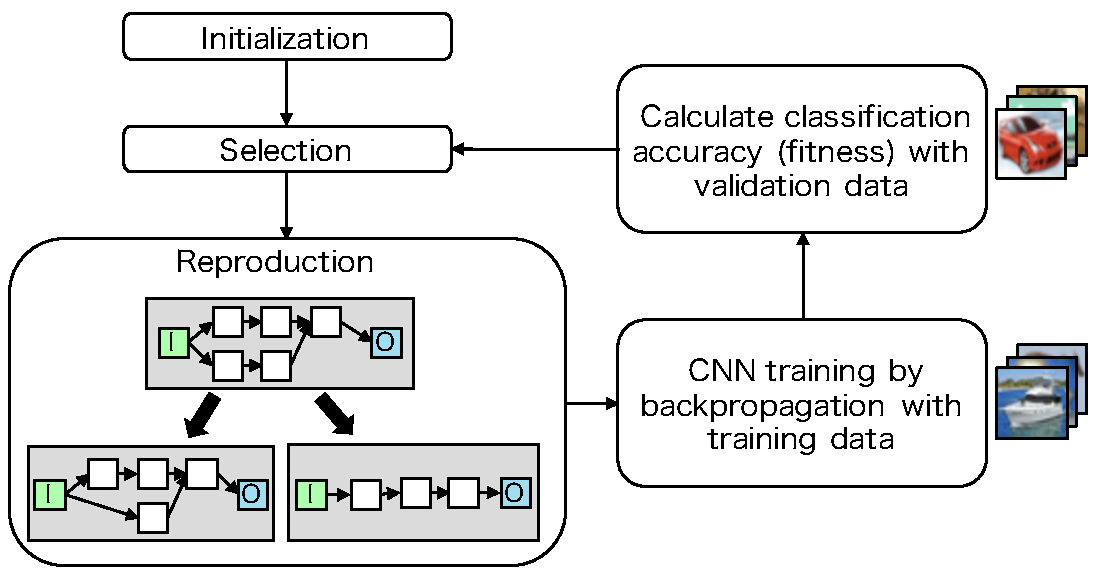
\includegraphics[width=0.99\linewidth, bb=0 0 526 276]{images/overview.pdf}
\caption{Overview of our method. Our method represents \new{CNN} architectures based on Cartesian genetic programming. The CNN architecture is trained on a learning task and assigned the validation accuracy of the trained model as the fitness. The evolutionary algorithm searches the better architectures.}
\label{overview}
\end{figure}

\begin{figure*}[t]
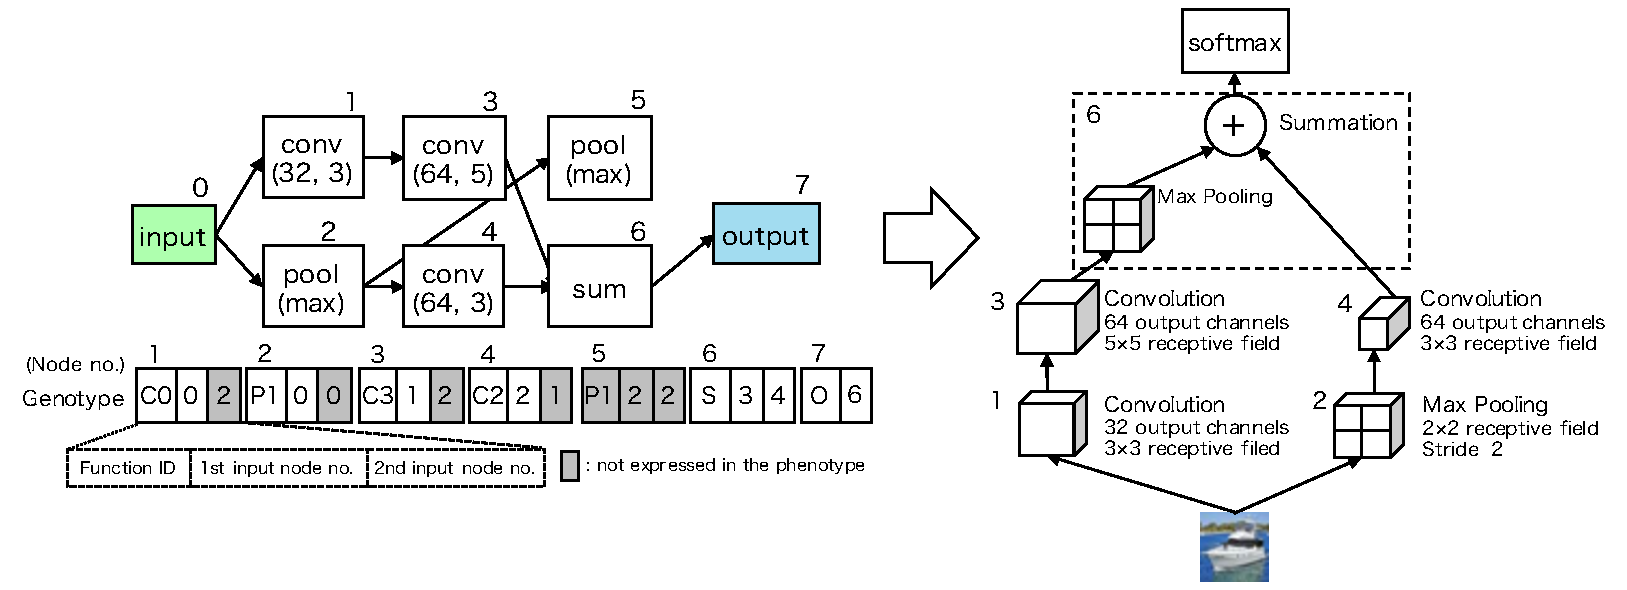
\includegraphics[width=0.99\linewidth, bb=0 0 781 283]{images/genotype.pdf}
\caption{Example of a genotype and a phenotype. The genotype (left) defines the CNN architecture (right). In this case, node No. 5 on the left side is \new{an inactive node.} The summation node performs \new{max pooling} to \new{the} first input so as to get the same input tensor sizes.}
\label{genotype}
\end{figure*}


% ----------------------------------------------------------------------------------------------------
\section{CNN Architecture Design Using Cartesian Genetic Programming}
Our method directly encodes the CNN architectures based on CGP \cite{harding_evolution_2008,miller_redundancy_2006,miller_cartesian_2000} and uses the \new{highly functional} modules as the node functions.
The CNN architecture defined by \new{CGP} is trained using \new{a} training dataset, \new{and} the validation accuracy is assigned as the fitness of the architecture. Then\new{,} the architecture is optimized to maximize the validation accuracy by the evolutionary algorithm.
Figure \ref{overview} illustrates \new{an} overview of our method.

In this section, we describe the network representation and the evolutionary algorithm used in the proposed method in detailed.

\subsection{Representation of CNN Architectures}
We use the CGP encoding scheme, representing the program as \new{directed} acyclic graphs with a two-dimensional grid defined on computational nodes, for the CNN architecture representation. Let \new{us} assume \new{that} the grid has $N_r$ rows by $N_c$ columns\new{;} then the number of intermediate nodes is $N_r \times N_c$, and the numbers of inputs and outputs depend on the task. The genotype consists of \new{integers} with fixed \new{lengths}, and each gene has \new{information} \new{regarding} the type and connections of the node. The $c$-th column's nodes should be connected from the $(c-l)$ to $(c-1)$-th column's nodes, where $l$ is called \new{the} levels-back parameter. Figure \ref{genotype} \new{provides} an example of the genotype, the corresponding network\new{,} and \new{the} CNN architecture in the case of two rows by three columns. \new{Whereas} the genotype in CGP is a \new{fixed-length} representation, the number of nodes in the phenotypic network varies \new{because} not all \new{of} the nodes are \new{connected} to the output nodes. \new{Node} No. 5 \new{on} the left \new{side} of Fig.~\ref{genotype} is \new{an} inactive \new{node.}

Referring \new{to} the modern CNN architectures, we select the \new{highly functional} modules as the node function.
The \new{frequently used} processings in the CNN are convolution and pooling; convolution processing uses a local connectivity and spatially shares the learnable weights, and pooling is nonlinear down-sampling.
We prepare the six types of node functions called ConvBlock, ResBlock, \new{max pooling, average pooling}, concatenation, and summation.
These nodes operate the \new{three-dimensional (3-D)} tensor defined by the dimensions of the row, column, and channel. Also, we call this 3-D tensor \nnew{feature maps}, where a feature map indicates a matrix of the row and column as \new{an} image plane.

The ConvBlock consists of \new{standard} convolution processing with \new{a} stride of 1 followed by batch normalization \cite{ioffe_batch_2015} and rectified linear units (ReLU) \cite{nair_rectified_2010}. In the ConvBlock, we pad the outside of input feature maps with zero values before the convolution operation so as to \new{maintain} the row and column sizes of the output. 
As a result, the $M \times N \times C$ input feature maps are transformed \new{into} $M \times N \times C'$ output ones, where $M$, $N$, $C$, and $C'$ are the numbers of rows, columns, input channels, and output channels, respectively.
We prepare several ConvBlocks with the different output channels and \new{the} receptive field size (kernel size) in the function set of CGP.

The ResBlock is composed of a convolution processing, batch normalization, ReLU, and tensor summation. A ResBlock architecture is shown in Fig.~\ref{resblock}.
The ResBlock performs identity mapping by shortcut connections as described in \cite{he_deep_2016}.
The row and column sizes of the input are preserved in the same way as ConvBlock after convolution.
The output feature maps of the ResBlock are calculated by the ReLU activation and the summation with the input feature maps and the processed feature maps as shown in Fig.~\ref{resblock}.
In the ResBlock, the $M \times N \times C$ input feature maps are transformed into the $M\times N\times C'$ output ones.
We also prepare several ResBlocks with the different output channels and \new{the} receptive field size in the function set of CGP.

\begin{figure}[t]
%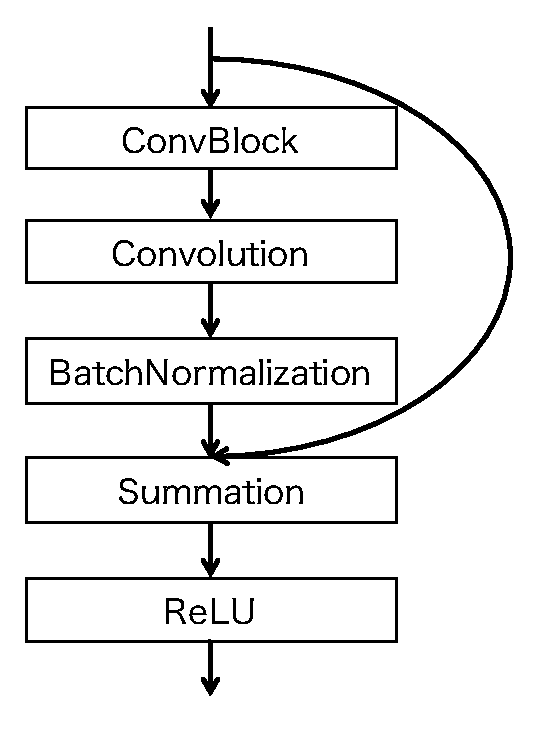
\includegraphics[scale=0.45]{images/resblock.eps}
\begin{center}
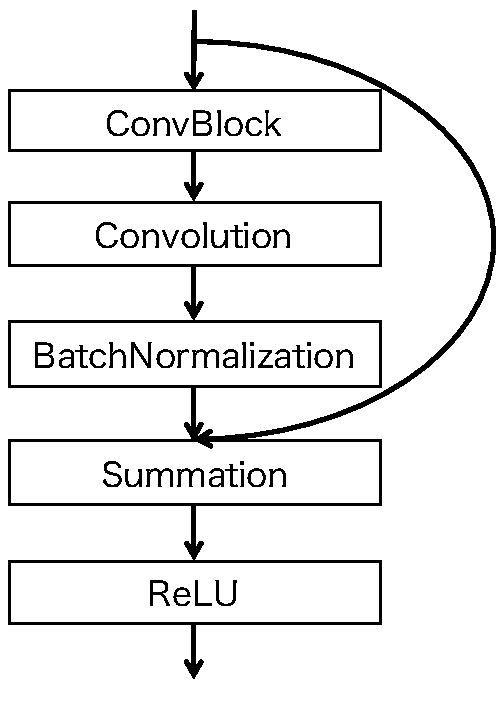
\includegraphics[scale=0.45, bb=0 0 242 339]{images/resblock.pdf}
\caption{ResBlock architecture.}
\label{resblock}
\end{center}
\end{figure}

The \new{max} and \new{average poolings} perform a max and average operation, respectively, over the local neighbors of the feature maps. We use the pooling with the $2 \times 2$ receptive field size and the stride size 2.
In the pooling operation, the $M \times N \times C$ input feature maps are transformed into the $M' \times N' \times C$ output ones, where $M' = \lfloor M/2 \rfloor$ and $N' = \lfloor N/2 \rfloor$.

The concatenation function concatenates two feature maps in the channel dimension.
If the input feature maps to be concatenated have \new{different} \new{numbers} of rows or columns, we down-sample the larger feature maps by \new{max pooling} so \new{that they} become the same sizes of \new{the} inputs.
In the concatenation operation, the \new{sizes} of the output feature maps are $\min (M_1, M_2) \times \min (N_1, N_2) \times (C_1 + C_2)$, where \new{as} the sizes of the inputs are $M_1 \times N_1 \times C_1$ and $M_2 \times N_2 \times C_2$.

The summation performs \new{the} element-wise addition of two feature maps, channel by channel. 
In the same way as the concatenation, if the input feature maps to be added have \new{different} \new{numbers} of rows or columns, we down-sample the larger feature maps by \new{max pooling.}
\new{In addition}, if the inputs have \new{different} \new{numbers} of channels, we pad the smaller feature maps with zeros for increasing channels.
In the summation operation, the size of the output feature maps are $\min (M_1, M_2) \times \min (N_1, N_2) \times \max (C_1, C_2)$, where the sizes of the inputs are $M_1 \times N_1 \times C_1$ and $M_2 \times N_2 \times C_2$. In Fig.~\ref{genotype}, the summation node performs \new{max pooling} to \new{the} first input so as to get the same input tensor sizes. Adding these summation and concatenation operations allows our method to represent shortcut connections or branching layers\new{,} such as \new{those} used in GoogleNet \cite{szegedy_going_2015} and Residual Net \cite{he_deep_2016} without \new{ResBlock.}

The output node represents \new{the} softmax function with the number of classes. The outputs fully connect to all elements of the input.
The node functions used in the experiments are displayed in Table \ref{tbl:node_func}.

\subsection{Evolutionary Algorithm}
We use a point mutation as the genetic operator in the same way as the standard CGP. The type and connections of each node randomly change to valid values according to a mutation rate. 
The standard CGP mutation has \new{the} possibility \new{of affecting only} the inactive node. In that case, the phenotype (representing \new{the} CNN architecture) does not change by the mutation and does not \new{require a} fitness evaluation again.

The fitness evaluation of the CNN architectures is so expensive \new{because} it requires the training of CNN.
To efficiently use the computational resource, we want to evaluate some candidate solutions in parallel at each generation.
Therefore, we apply the mutation operator until at least one active node changes for reproducing the candidate solution. We call this mutation \new{a} forced mutation.
Moreover, to \new{maintain} a neutral drift, which is effective for CGP evolution \cite{miller_redundancy_2006,miller_cartesian_2000}, we modify a parent by the neutral mutation if the fitnesses of the offsprings do not improve.
Here, the neutral mutation \new{changes} \new{only} the genes of \new{the} inactive nodes without \new{the} modification of the phenotype.

We use the modified $(1+\lambda)$ evolutionary strategy (with $\lambda = 2$ in our experiments) \new{in} the above artifice.
The procedure of our modified algorithm is as follows:
\begin{enumerate}
  \item Generate an initial individual at random as \new{parent $P$,} and train the CNN represented by $P$ followed by assigning the validation accuracy as the fitness.
  \item Generate a set of $\lambda$ offsprings $C$ by applying the forced mutation to $P$.
  \item Train the $\lambda$ CNNs represented by offsprings $C$ in parallel\new{,} and assign the validation accuracies as the fitness.
  \item Apply the neutral mutation to \new{parent} $P$.
  \item Select an elite individual from the set of $P$ and $C$\new{,} and then replace $P$ with the elite individual.
  \item Return to step $2$ until a stopping criterion is satisfied.
\end{enumerate}

\begin{table}[tb]
\caption{The node functions and abbreviated symbols used in the experiments.}
\label{tbl:node_func}
\begin{tabular}{l|l|l} \hline
Node type & Symbol & Variation \\ \hline
ConvBlock & CB ($C'$, $k$) & $C' \in \{32, 64, 128\}$ \\
                 &                      & $k \in \{ 3\times3, 5 \times 5 \}$ \\
ResBlock   & RB ($C'$, $k$) & $C' \in \{32, 64, 128\}$ \\
                 &                      & $k \in \{ 3 \times 3, 5 \times 5 \}$ \\
\new{Max pooling}       & MP              & -- \\
\new{Average pooling} & AP              & -- \\
Summation      & Sum     & -- \\
Concatenation & Concat & -- \\ \hline
\multicolumn{3}{l}{$C'$: Number of output channels} \\
\multicolumn{3}{l}{$k$: Receptive field size (kernel size)}
\end{tabular}
\end{table}

% ----------------------------------------------------------------------------------------------------
\section{Experiments and Results}
\subsection{Dataset}
We test our method on the image classification task using the CIFAR-10 dataset in which the number of classes is $10$. The numbers of training and test images are $50,000$ and $10,000$, respectively, and the size of images is $32 \times 32$.

We consider two experimental scenarios: \new{the} default scenario and \new{the} small-data scenario.
The default scenario uses the default numbers of the training images, \new{whereas} the small-data scenario assumes that we \new{use only $5,000$} images as the learning data. 

In the default scenario, we randomly \new{sample} $45,000$ images from the training set to train the CNN\new{,} and \new{we} use the remaining $5,000$ images for the validation set of the CGP fitness evaluation.
In the small-data scenario, we randomly \new{sample} $4,500$ images for the training and $500$ images for the validation.

\subsection{Experimental Setting}

\begin{table}[t]
  \caption{Parameter setting for the CGP}
  \label{cgp_param}
  \begin{tabular}{l|l} \hline
    Parameters & Values \\ \hline
%   \# Generations & $300$ (default scenario) \\ 
%                          & $2000$ (small-data scenario) \\ 
   Mutation rate & $0.05$ \\
   \#  Rows ($N_r$) & $5$ \\
   \#  Columns ($N_c$) & $30$ \\
   Levels-back ($l$) & $10$ \\ \hline
  \end{tabular}
\end{table}


To assign the fitness to the candidate CNN architectures, we train the CNN by stochastic gradient descent (SGD) with \new{a} mini-batch size of $128$. The softmax \new{cross-entropy} loss is used as the loss function.
We initialize the weights by the He's method \cite{he_delving_2015} and use the Adam optimizer \cite{kingma_adam:_2015} with an initial learning rate of $0.01$. 
We train each CNN for 50 epochs and reduce the learning rate by a factor of 10 at 30th epoch.

We preprocess the data with the per-pixel mean subtraction.
To prevent overfitting, we use a weight decay with the coefficient $1.0 \times 10^{-4}$ and data augmentation.
We use the data augmentation method based on \cite{he_deep_2016}: padding $4$ pixels on each side followed by choosing a random $32\times 32$ crop from the padded image, and random horizontal flips on the cropped $32 \times 32$ image.

The parameter setting for \new{CGP} is shown in Table \ref{cgp_param}. We use the relatively larger number of columns than the number of rows to generate deep architectures \new{that are} likely.
The offspring size \new{of} $\lambda$ is set to two\new{;} that is the same number of GPUs in our experimental machines.
We test two node function sets called ConvSet and ResSet for our method.
The ConvSet contains ConvBlock,  \new{Max pooling, Average pooling}, Summation, and Concatenation in Table \ref{tbl:node_func}, and the ResSet contains ResBlock,  \new{Max pooling, Average pooling}, Summation, and Concatenation.
The difference between these two function sets is whether we adopt ConvBlock or ResBlock.
The numbers of generations are \nnew{$500$ for ConvSet, $300$ for ResSet in the default scenario, and $1,500$ in the small-data scenario}, respectively.

After the CGP process, we re-train the best CNN architecture using each training \new{image} ($50,000$ for the default scenario and $5,000$ for the small-data scenario)\new{,} and \new{we} calculate the classification accuracy for the $10,000$ test images to evaluate the constructed CNN architectures.

%In this re-training phase, we optimize the weights of the obtained architecture with a different training schedule; we set a learning rate to $0.01$ during \new{the} first $50$ epochs and then reduce \new{it} to $0.001$ during \new{the} subsequent $50$ epochs. The other parameters are \new{the} same as \new{those} used in the CGP process.
\nnew{In this re-training phase, we optimize the weights of the obtained architecture for $500$ epochs with a different training procedure; we use} \nnew{SGD with a momentum of $0.9$, a mini-batch size of $128$, and a weight decay of $5.0 \times 10^{-4}$.}
\nnew{We start a learning rate of $0.01$ and set it to $0.1$ at $5$th epoch, then we reduce it to $0.01$ and $0.001$ at $250$th and $375$th epochs, respectively. This learning rate schedule is based on the reference \cite{he_deep_2016}.}

We \new{have} implemented our methods using the Chainer \cite{tokui_chainer:_2015} (version 1.16.0) framework and \new{run} the experiments on the machines with $3.2$GHz CPU, $32$GB RAM, and two NVIDIA GeForce GTX 1080 (or two GTX 1070) GPUs.
\new{It is possible that the large architectures generated by the CGP process cannot run in the environment} \nnew{due to the GPU memory limitation.}
In that case, we assign a zero fitness to the candidate solution.

\begin{figure*}[t]
 \begin{minipage}[b]{0.45\linewidth}
  \centering
  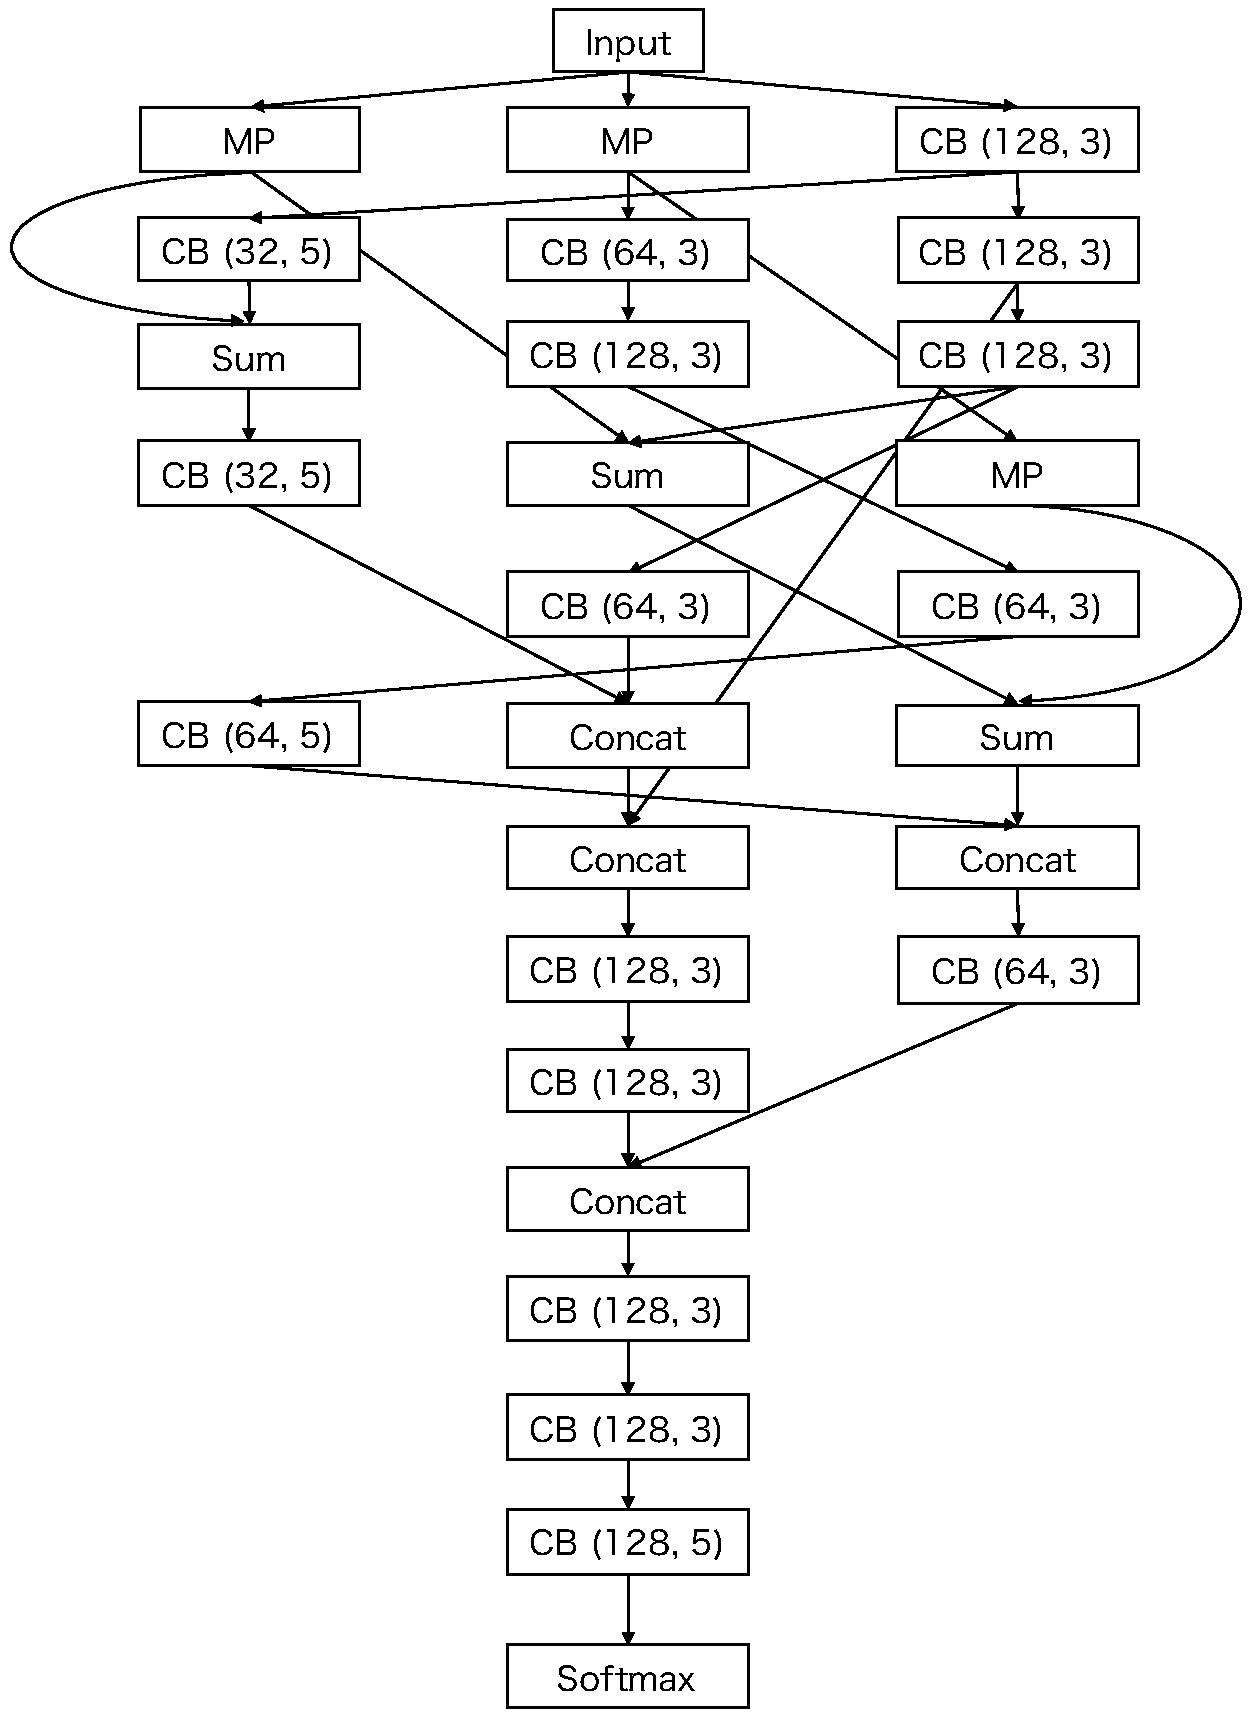
\includegraphics[keepaspectratio, scale=0.4, bb=0 0 600 827]{images/modelA.pdf}
  \subcaption{CGP-CNN (ConvSet)}\label{modelA}
 \end{minipage}
 \begin{minipage}[b]{0.45\linewidth}
  \centering
  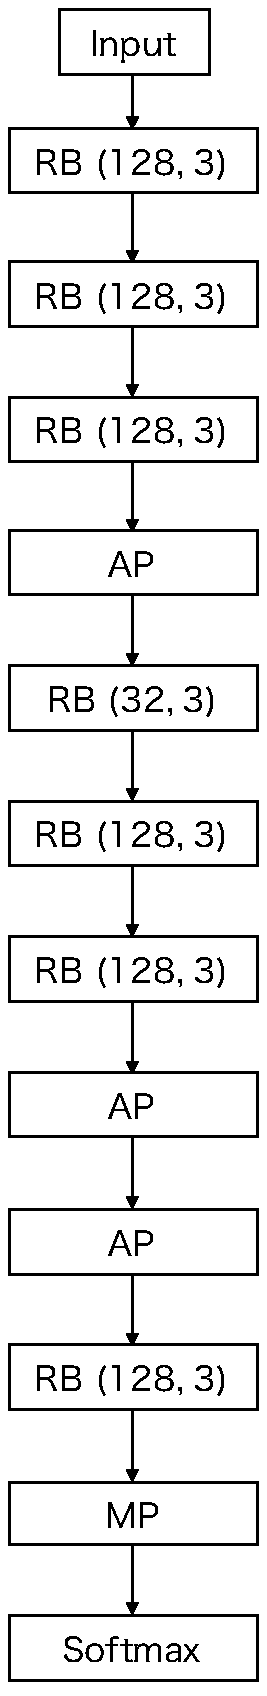
\includegraphics[keepaspectratio, scale=0.4, bb=0 0 128 814]{images/modelB.pdf}
  \subcaption{CGP-CNN (ResSet)}\label{modelB}
 \end{minipage}
 \caption{The CNN architectures designed by our method on the default scenario.}\label{models}
\end{figure*}

%\begin{figure*}[!t]
%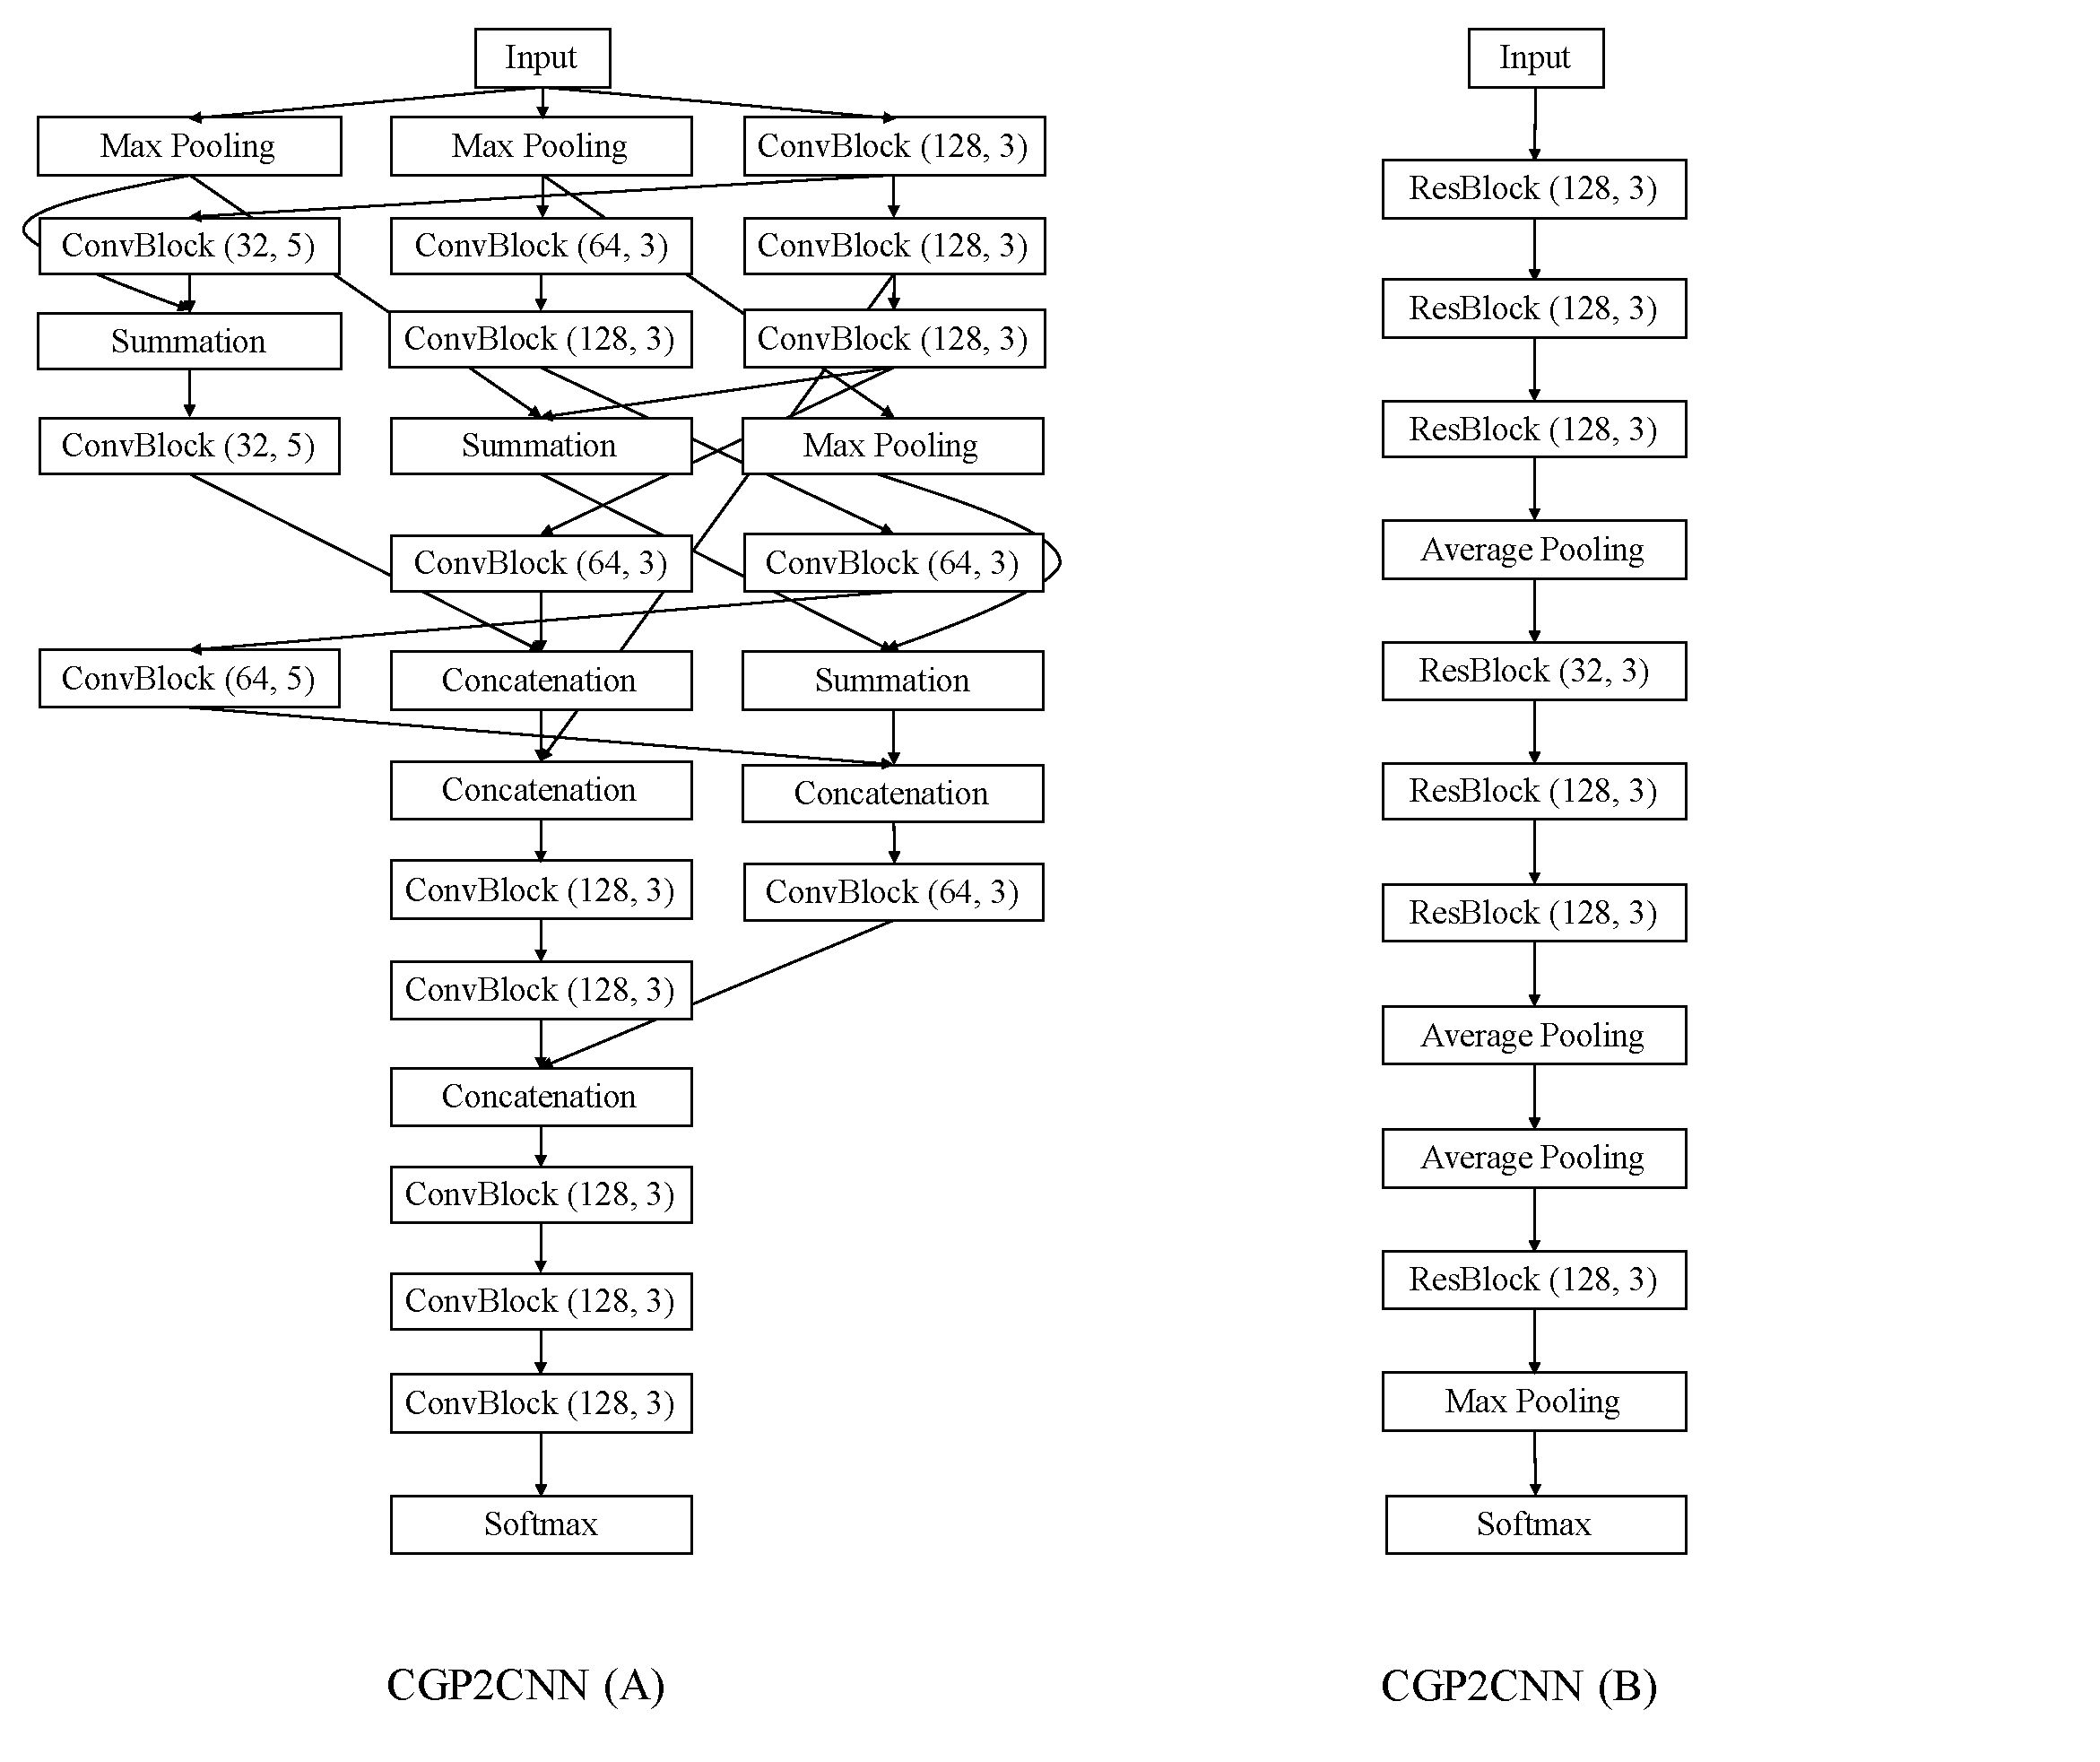
\includegraphics[scale=0.48]{images/models.eps}
%\caption{CNN architectures designed by our method. $ConvBlock(n, k)$ denotes a ConvBlock node with $n$ filters and receptive field size $k$. $ResBlock(n, k)$ denotes a ResBlock node with $n$ filters and receptive field size $k$.}
%\label{models}
%\end{figure*}

%\begin{figure}[!t]
%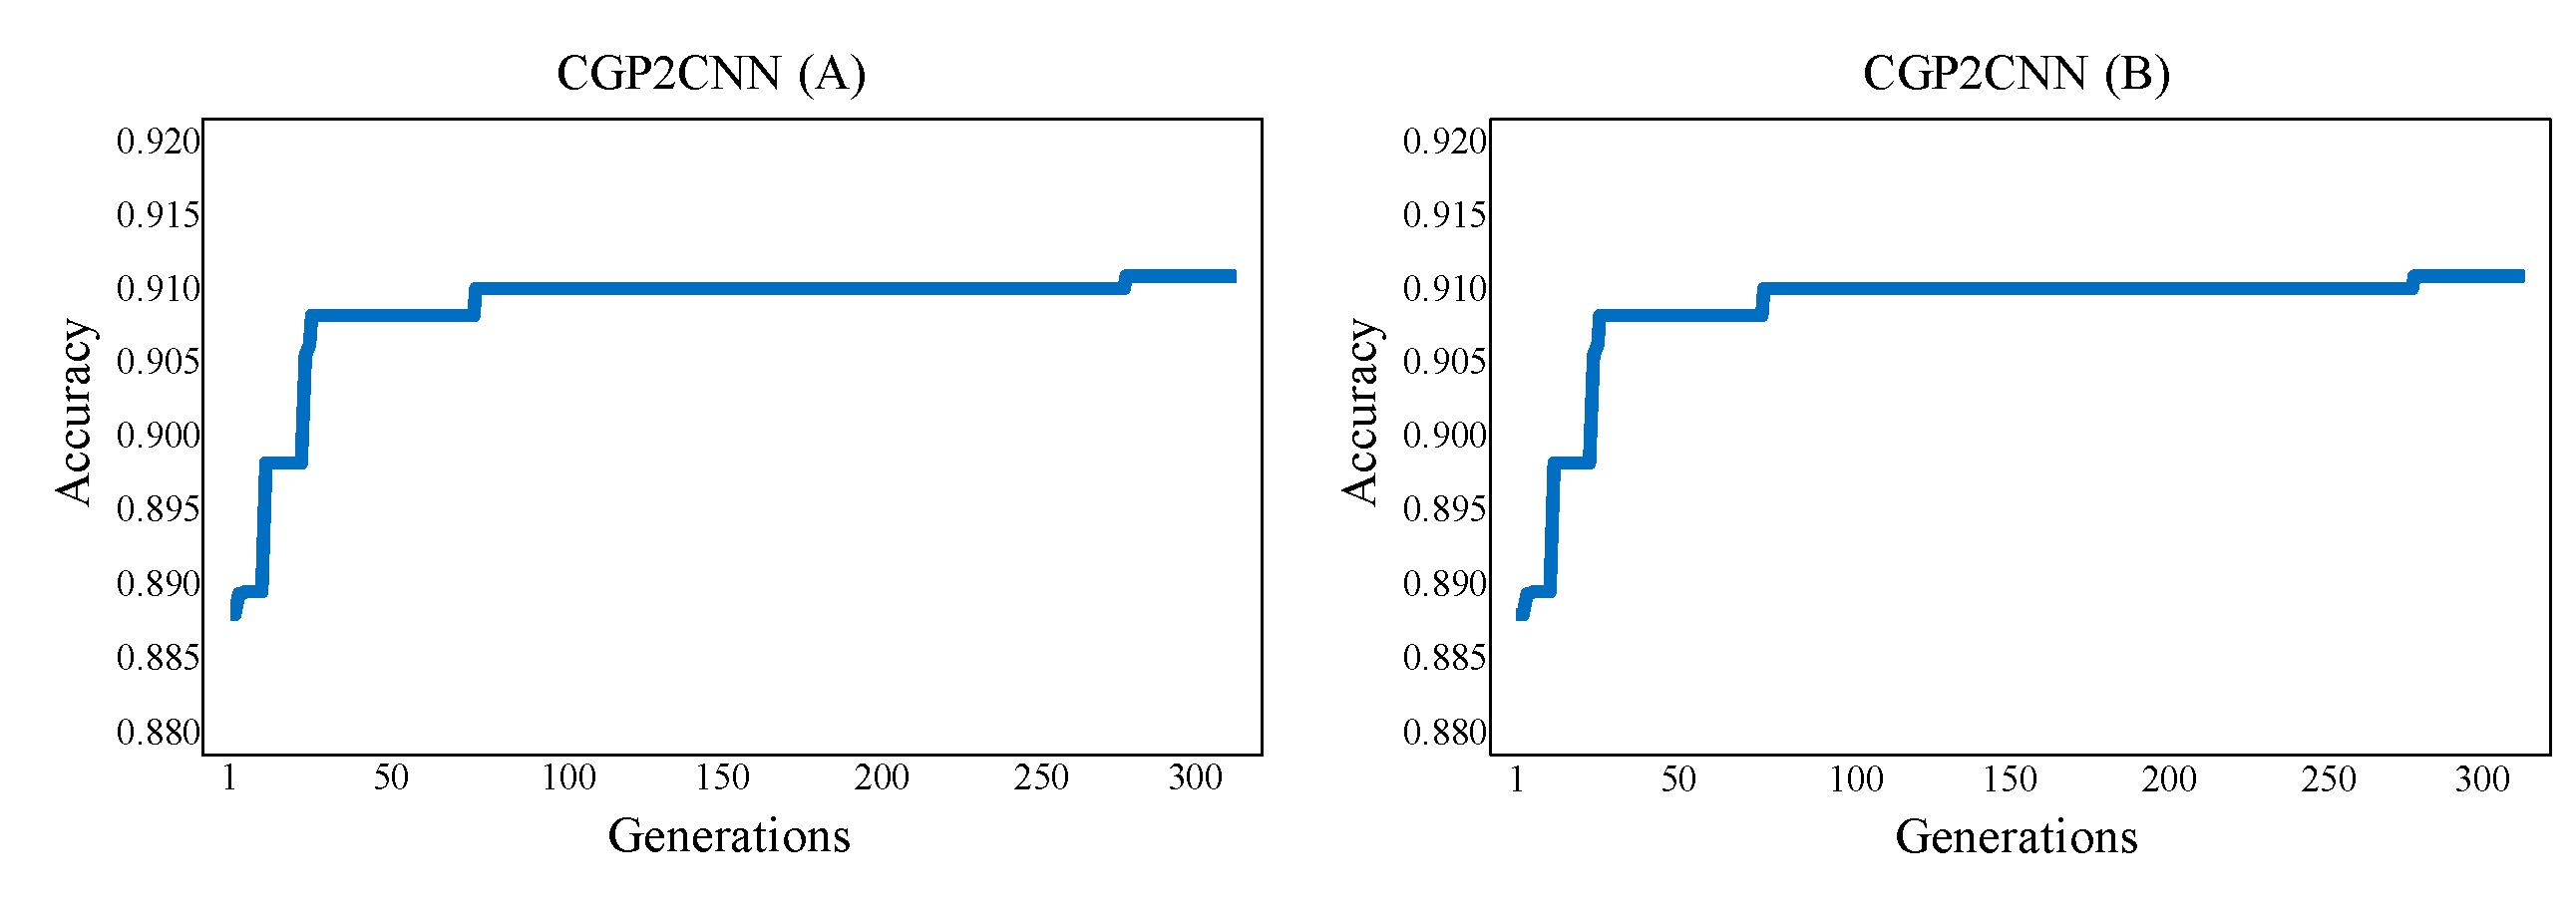
\includegraphics[scale=0.19]{images/fitness.eps}
%\caption{Transition of the fitness of CGP2CNN (A) and CGP2CNN (B).}
%\label{fitness}
%\end{figure}

\subsection{Result of the Default Scenario}
We compare the classification performance of our method with the state-of-the-art methods and summarize the classification error rates in Table \ref{results}. We refer to the architectures constructed by the proposed method as CGP-CNN. For instance, CGP-CNN (ConvSet) means the proposed method with \new{the} node function set of ConvSet. The models, Maxout, Network in Network, VGG, and ResNet, are hand-crafted CNN architectures, \new{whereas} the MetaQNN and Neural Architecture Search are the models constructed by the \new{reinforcement learning-based method.}
In Table \ref{results}, the numbers of learnable weight parameters in the models are also listed.

\begin{table}[t]
  \caption{Comparison of error rates on the CIFAR-10 dataset (default scenario). The values of Maxout, Network in Network, ResNet, MetaQNN, and Neural Architecture Search are referred from the reference papers.}
  \label{results}
  \begin{tabular}{l|c|c} \hline
   Model & Error rate & \# params ($\times 10^6$) \\ \hline
   Maxout \cite{goodfellow_maxout_2013} & $9.38$ & -- \\ 
   Network in Network \cite{lin_network_2014} & $8.81$ & -- \\
   VGG \cite{simonyan_very_2014} \footnotemark & $7.94$ & $15.2$ \\
   ResNet \cite{he_deep_2016} & $6.61$ & $1.7$ \\
   MetaQNN \cite{baker_designing_2016} \footnotemark & $9.09$ & $3.7$ \\
   Neural Architecture Search \cite{zoph_neural_2016} & $3.84$ & $32.0$ \\
   CGP-CNN (ConvSet) & $6.75$ & $1.52$ \\
   CGP-CNN (ResSet) & $5.98$ & $1.68$ \\ \hline
   %\multicolumn{1}{l}{*The mean error rate and the number of parameters of top $5$ models.} & \multicolumn{1}{l}{} & \multicolumn{1}{l}{} \\
  \end{tabular}
\end{table}
\footnotetext[1]{We \new{have} implemented the VGG net \cite{simonyan_very_2014} for the CIFAR-10 dataset \new{because} the VGG net is not applied to the CIFAR-10 dataset in \cite{simonyan_very_2014}. The architecture of the VGG is identical with  \new{configuration} D in \cite{simonyan_very_2014}. We denote this model as VGG in this paper.}
\footnotetext[2]{The mean error rate and the number of parameters of \new{the} top \new{five} models are shown.}


As can be seen in Table \ref{results}, the error rates of our methods are competitive with the state-of-the-art methods.
In particular, CGP-CNN (ResSet) outperforms all hand-crafted models, and the \new{architectures constructed} by \new{using} our method have a good balance between classification \new{errors} and the number of parameters. The Neural Architecture Search achieved the best error rate\new{,} but this method used 800 GPUs for the architecture search. Our method could find a competitive architecture with \new{a} reasonable machine resource.

Figure \ref{models} shows the architectures constructed by CGP-CNN (ConvSet) and CGP-CNN (ResSet). We can observe that these architectures are quite different; the summation and concatenation nodes are not used in CGP-CNN (ResSet), whereas these nodes \new{are} frequently used in CGP-CNN (ConvSet). These nodes lead the wide network; therefore\new{,} the network of CGP-CNN (ConvSet) is \new{a} wider structure than that of CGP-CNN (ResSet).

Added to this, we observe that \new{CGP-CNN (ResSet)} architecture has a similar feature with the ResNet \cite{he_deep_2016}. The ResNet consists of a repetition of two types of modules: the module \new{with} several convolutions with the shortcut connections without down-sampling, and down-sampling convolution with \new{a} stride of $2$.  Although our method cannot perform down-sampling in the ConvBlock and the ResBlock, we can see from Fig.~\ref{models} that CGP-CNN (ResSet) uses average pooling as an alternative to the down-sampling convolution. Furthermore, \new{CGP-CNN (ResSet)} has some convolutions with the shortcut \new{connections,} \new{such as} \new{ResNet.} Based on these observations, we can say that our method can also find the architecture similar to one designed by human experts, and that model shows a better performance.

Besides, while the ResNet has a very deep $110$-layer architecture, \new{CGP-CNN (ResSet)} has a relatively shallow and wide architecture.
We guess from this result that the number of output channels of \new{ResBlock} in the \new{proposed method} is one of the contributive parameters for improving the classification accuracy on the CIFAR-10 dataset.
%To investigate the effectiveness of the number of output channels, we change the number of output channels of ConvBlock in \new{CGP-CNN (ConvSet)} from $\{32, 64, 128\}$ to $\{64, 128, 256, 512\}$. We \new{have run} this modified version of the proposed method by \new{the} 150th generation. \shin{It may change...} \new{It has achieved an} error rate \new{of} $7.25$\% and \new{has} obtained \new{a shallower and wider} architecture.

%The fitness transition of CGP2CNN (A) and CGP2CNN (B) is shown in Figure \ref{fitness}.
%While the fitness remains flat from $100$ generation to $250$ generation, the improvement of the fitness is seen in about $300$ generation.
%It is likely that our method shows a better classification performance if we train the CGP in more generations.

\subsection{Result of the Small-data Scenario}
%For settings of our method, we changed the number of generation to $2,000$. The other experimental settings are the same in the preceding section.
In the small-data scenario, we compare our method with \new{VGG} and ResNet.
%For \new{VGG}, we \new{have} trained the model for 200 epochs using 5,000 training data by SGD with an initial learning rate of 0.01\new{,} and \new{we have} reduced the learning rate by a factor of 10 every 50 epochs.
\nnew{We have trained \new{VGG} and ResNet models by the same setting of the re-training method in the proposed method; it is based on the training method of the ResNet \cite{he_deep_2016}.}
%we \new{have} trained the model for 500 epochs using 5,000 training data by SGD and started with a learning rate of $0.1$, and then\new{, we have} divided it by \new{$10$} at 250 and 375 epochs. This learning rate schedule is described in \cite{he_deep_2016}.

Table 4 shows the comparison of error rates \new{in} the small-data scenario. We observe that our methods, CGP-CNN (ConvSet) and CGP-CNN (ResSet), can find better architectures than \new{VGG} and ResNet.
It is obvious that \new{VGG} and ResNet are inadequate for the small-data scenario \new{because} these architectures are designed for \new{a} relatively large amount of data. \new{Meanwhile}, our method can tune the architecture depending on the data size.
Figure \ref{model_small} illustrates the CGP-CNN (ConvSet) architecture constructed by \new{using} the proposed method.
As seen in Fig.~\ref{model_small}, our method \new{has found a} wider structure than that in the default scenario.

Additionally, we \new{have} re-trained this model with the $50,000$ training data and achieved \new{a} \nnew{$8.05\%$} error rate on the test data. It suggests that the proposed method \new{may be used} to design a relatively good general architecture even with a small dataset.


\begin{table}[t]
  \caption{Comparison of error rates on the CIFAR-10 dataset (small-data scenario).}
  \label{results_small}
  \begin{tabular}{l|c|c} \hline
   Model & Error rate & \# params ($\times 10^6$) \\ \hline
   VGG \cite{simonyan_very_2014} & $\nnew{24.11}$ & 15.2 \\
   ResNet \cite{he_deep_2016} & $24.10$ & 1.7 \\ 
   CGP-CNN (ConvSet) & $23.48$  & $3.9$  \\
   CGP-CNN (ResSet) & $23.47$ & $0.83$ \\ \hline
  \end{tabular}
\end{table}


% ----------------------------------------------------------------------------------------------------
\section{Conclusion}
In this paper, we have attempted to \new{take} a GP-based approach for designing the CNN architectures and \new{have} verified its potential.
The proposed method constructs the CNN architectures based on CGP and adopts the \new{highly functional} modules\new{,} such as ConvBlock and ResBlock\new{,} \new{for searching} the adequate architectures efficiently.
We \new{have} constructed the CNN architecture for the image classification task with the CIFAR-10 dataset and considered two different data size settings. The experimental result showed that the proposed method could automatically find the competitive CNN architecture compared with \new{the} state-of-the-art models.

However, our proposed method requires much computational cost; the experiment on the default scenario needed about \new{a} few weeks in our machine resource. We can reduce the computational time if the training data \new{are} small (\new{such as in} the small-data scenario in the experiment). Thus, one direction of future work is to develop the evolutionary algorithm to reduce the computational cost of the architecture design, e.g., increasing the training data for the neural network as the generation progresses. Another future work is to apply the proposed method to other image \new{datasets} and tasks.

\begin{figure}[t]
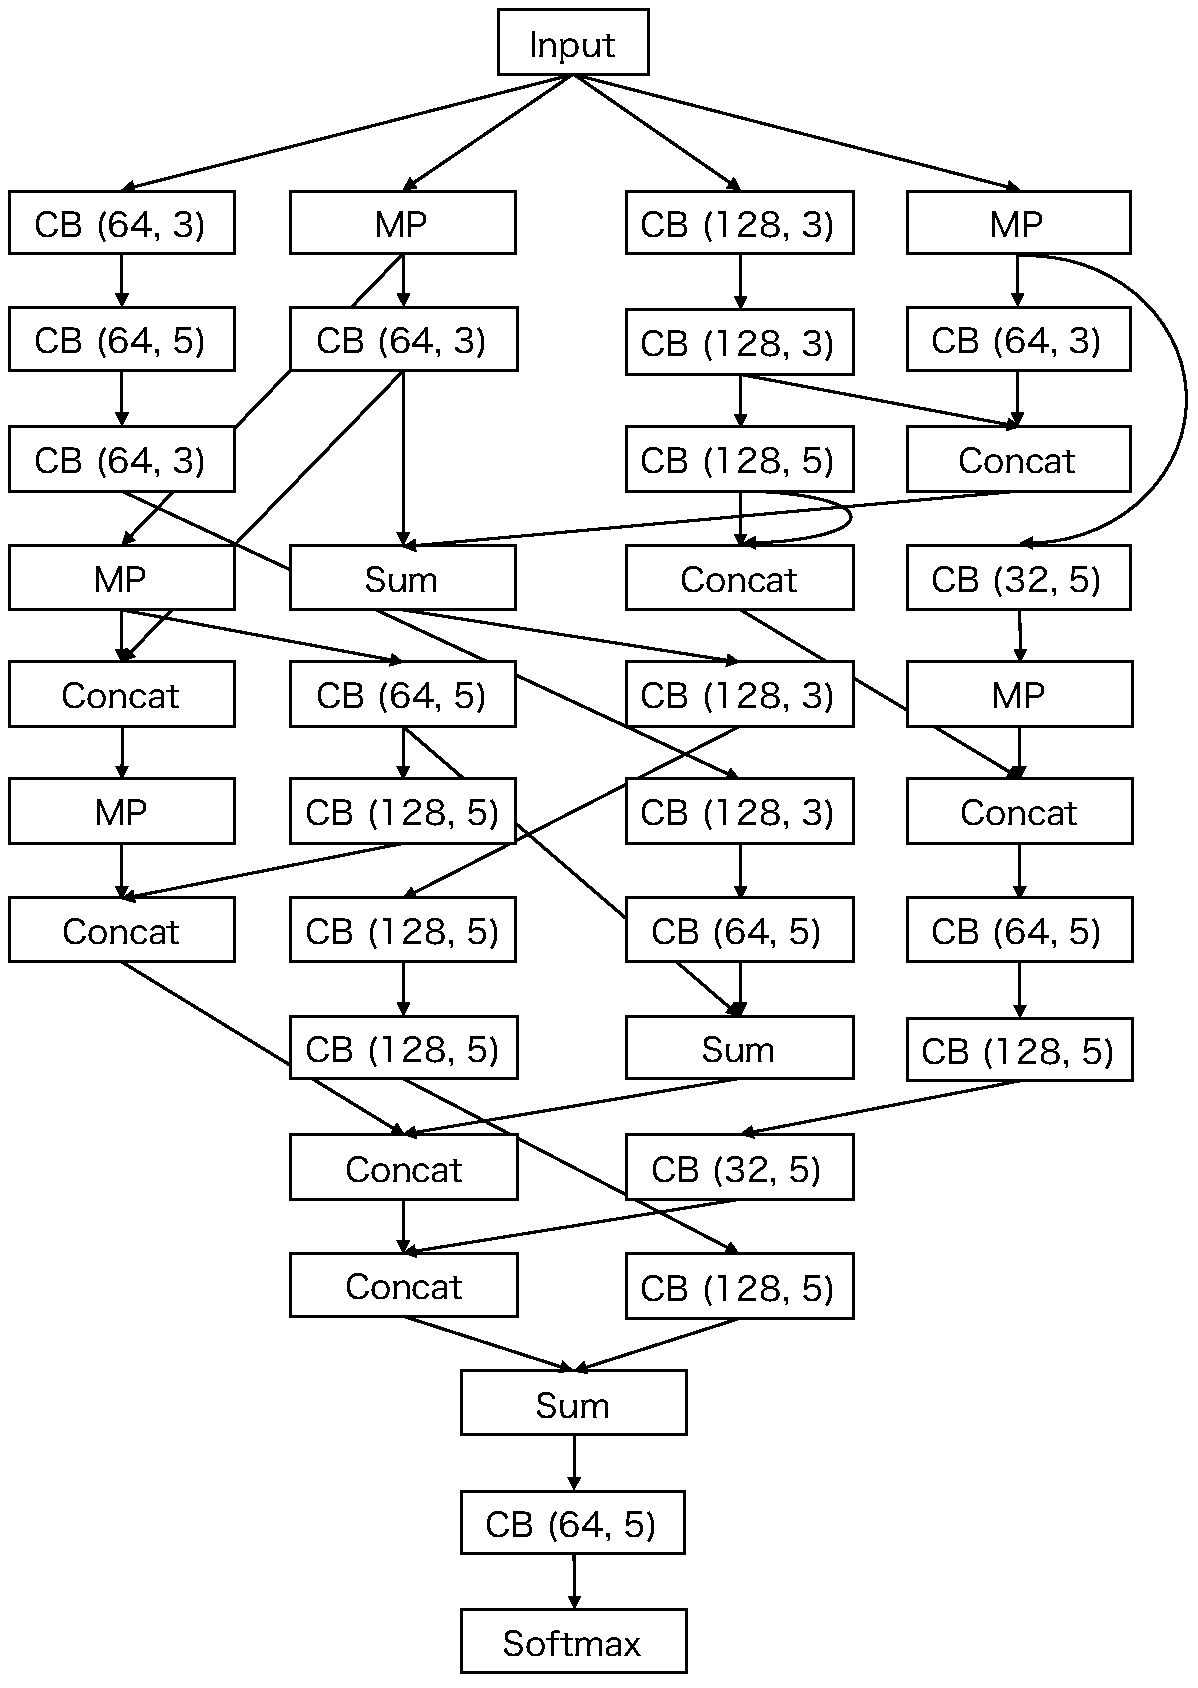
\includegraphics[width=0.9\linewidth, bb=0 0 575 810]{images/model_small.pdf}
\caption{The architecture of CGP-CNN (ConvSet) constructed \new{in} the small-data scenario.}
\label{model_small}
\end{figure}

